\documentclass[11pt, a4paper, singlecolumn, copyright, goog]{google}

\usepackage[authoryear, sort&compress, round]{natbib}
\newcounter{noteZZctr} \setcounter{noteZZctr}{1}
\newcommand{\ZZ}[1]{\textit{\textcolor{orange}{{{ZZ: \#\arabic{noteZZctr}: }}#1}} \addtocounter{noteZZctr}{1}}
\newcounter{noteWuctr} \setcounter{noteWuctr}{1}
\newcommand{\Wu}[1]{\textit{\textcolor{red}{{{Wu: \#\arabic{noteWuctr}: }}#1}} \addtocounter{noteWuctr}{1}}
\bibliographystyle{abbrvnat}
\usepackage[most]{tcolorbox}
\usepackage{pgfplots}
\usepackage{booktabs}
\usepackage{graphicx}
\usepackage{subcaption}
\usepackage{tikz}
\usepackage{makecell}
\usepackage{fontawesome5}
\usepackage{xcolor}
\usepackage{hyperref}
\usepackage{wrapfig}

\usepackage{listings}
\usepackage{xcolor}

\lstset{
  inputencoding=utf8,
  extendedchars=true,
  literate=
    {—}{{---}}1
    {–}{{--}}1
    {×}{{$\times$}}1
    {→}{{$\rightarrow$}}2
    {“}{{``}}1
    {”}{{''}}1
    {‘}{{`}}1
    {’}{{'}}1
}

\definecolor{promptbg}{gray}{0.97}
\definecolor{promptgray}{gray}{0.45}

\lstdefinestyle{promptstyle}{
    basicstyle=\ttfamily\scriptsize,
    backgroundcolor=\color{promptbg},
    commentstyle=\color{promptgray},
    numbers=left,
    numberstyle=\tiny\color{promptgray},
    numbersep=6pt,
    breaklines=true,
    breakatwhitespace=false,
    showstringspaces=false,
    keepspaces=true,
    columns=fullflexible,
    tabsize=2,
    frame=single,
    rulecolor=\color{black!20},
    xleftmargin=1.5em,
    framexleftmargin=1.2em
}

\usepackage{listings}
\usepackage{xcolor}



\definecolor{codegray}{gray}{0.45}
\definecolor{codebg}{gray}{0.97}

\lstdefinestyle{appendixcode}{
    basicstyle=\ttfamily\scriptsize,
    backgroundcolor=\color{codebg},
    commentstyle=\color{codegray},
    numbers=left,
    numberstyle=\tiny\color{codegray},
    numbersep=6pt,
    breaklines=true,
    breakatwhitespace=false,
    showstringspaces=false,
    keepspaces=true,
    columns=fullflexible,
    tabsize=2,
    frame=single,
    rulecolor=\color{black!20},
    xleftmargin=1.5em,
    framexleftmargin=1.2em
}

\newtcolorbox{taskbox}[1]{
  enhanced,
  colback=black!2,
  colframe=black!25,
  boxrule=0.6pt,
  arc=1.5mm,
  left=2.2mm,
  right=2.2mm,
  top=1.8mm,
  bottom=1.8mm,
  title={\textbf{#1}},
  coltitle=black,
  colbacktitle=black!5,
  fonttitle=\small
}

% Remove these if they are not needed
% \paperurl{https://arxiv.org/abs/123}

% comment out if logo should not be used
\uselogo{} 

\title{Dream-RSI: Recursive Self-Improvement through Evolving Worlds}


% Can leave this option out if you do not wish to add a corresponding author.
\correspondingauthor{xidongwu@google.com, zzhangx@google.com}

% Use the internally issued paper ID, if available
% \reportnumber{0001} % Leave blank if n/a

% Assign your own date to the report.
% Can comment out if not needed or leave blank if n/a.
\renewcommand{\today}

% Can have as many authors and as many affiliations as needed. Best to indicate joint
% first-authorship as shown below.
\author[1,2]{Tong Zheng}
\author[1]{Xidong Wu}
\author[1]{Zheng Zhang}
\author[3]{Zhankui He}
\author[1]{Chaoyi Zhang}
\author[3]{Benjamin Coleman}
\author[1]{Ruoqiao Wei}
\author[3]{Di Bai}
\author[4]{Haolin Liu}
\author[2]{Rui Liu}
\author[1]{Xue Wang}
\author[1]{Yue Zhuan}
\author[3]{Wang-Cheng Kang}
\author[1]{Renkai Xiang}
\author[2]{Heng Huang}
\author[1]{Xinwu Cheng}
\author[1]{Yunsong Guo}


% Affiliations *must* come after the declaration of \author[]
% \affil[*]{Equal contributions}
\affil[1]{\thepa{}{}}
\affil[2]{University of Maryland, College Park}
\affil[3]{Google Deepmind}
\affil[4]{University of Virginia}
\begin{abstract}
Recursive self-improvement is becoming increasingly vital for autonomous AI agents, where progress hinges on discovering high-value solutions across complex domains. The driver of this process is effective exploration, however, managing and improving exploration strategies remains a major bottleneck. Current systems face a fundamental dilemma: fixed strategies fail to adapt as search spaces scale, while online policy optimization requires navigating vast meta-search spaces under delayed and expensive feedback over long-horizon rollouts. We introduce \textsc{Dream-RSI}, a framework for scalable and recursively self-improving exploration. A lightweight orchestration layer makes exploration explicit and programmable while leaving the underlying coding agent unchanged. Our key insight is that accumulated discovery history can serve as a replay simulator over the realized search space. By performing dreaming in the replay simulator constructed from historical discovery trees, \textsc{Dream-RSI} secures immediate, low-cost off-policy feedback to evaluate and refine exploration policies without invoking repetitive, expensive online evaluations. The improved policy is subsequently redeployed online to drive further discovery, continuously expanding the simulator pool in a self-improving loop. Across algorithm engineering, mathematical optimization, and GPU kernel engineering, \textsc{Dream-RSI} achieves competitive or improved discovery quality while substantially reducing discovery cost in several settings.

\par\vspace{0.6em}
{\centering
\href{https://github.com/zhengkid/Dream-RSI}{%
\raisebox{-0.12em}{\Large\color{black}\faGithub}\hspace{0.35em}%
{\small\ttfamily\color{blue}github.com/zhengkid/Dream-RSI}%
}
\hspace{1.5em}\textcolor{gray}{|}\hspace{1.5em}% 分隔符
\href{https://dream-rsi.com/}{%
\raisebox{-0.12em}{\Large\color{black}\faGlobe}\hspace{0.35em}%
{\small\ttfamily\color{blue}dream-rsi.com}%
}
\par}
\end{abstract}

\begin{document}

\maketitle

\section{Introduction}

% \input{Main_Text/Figures/teasar}

\begin{figure}
    \centering
    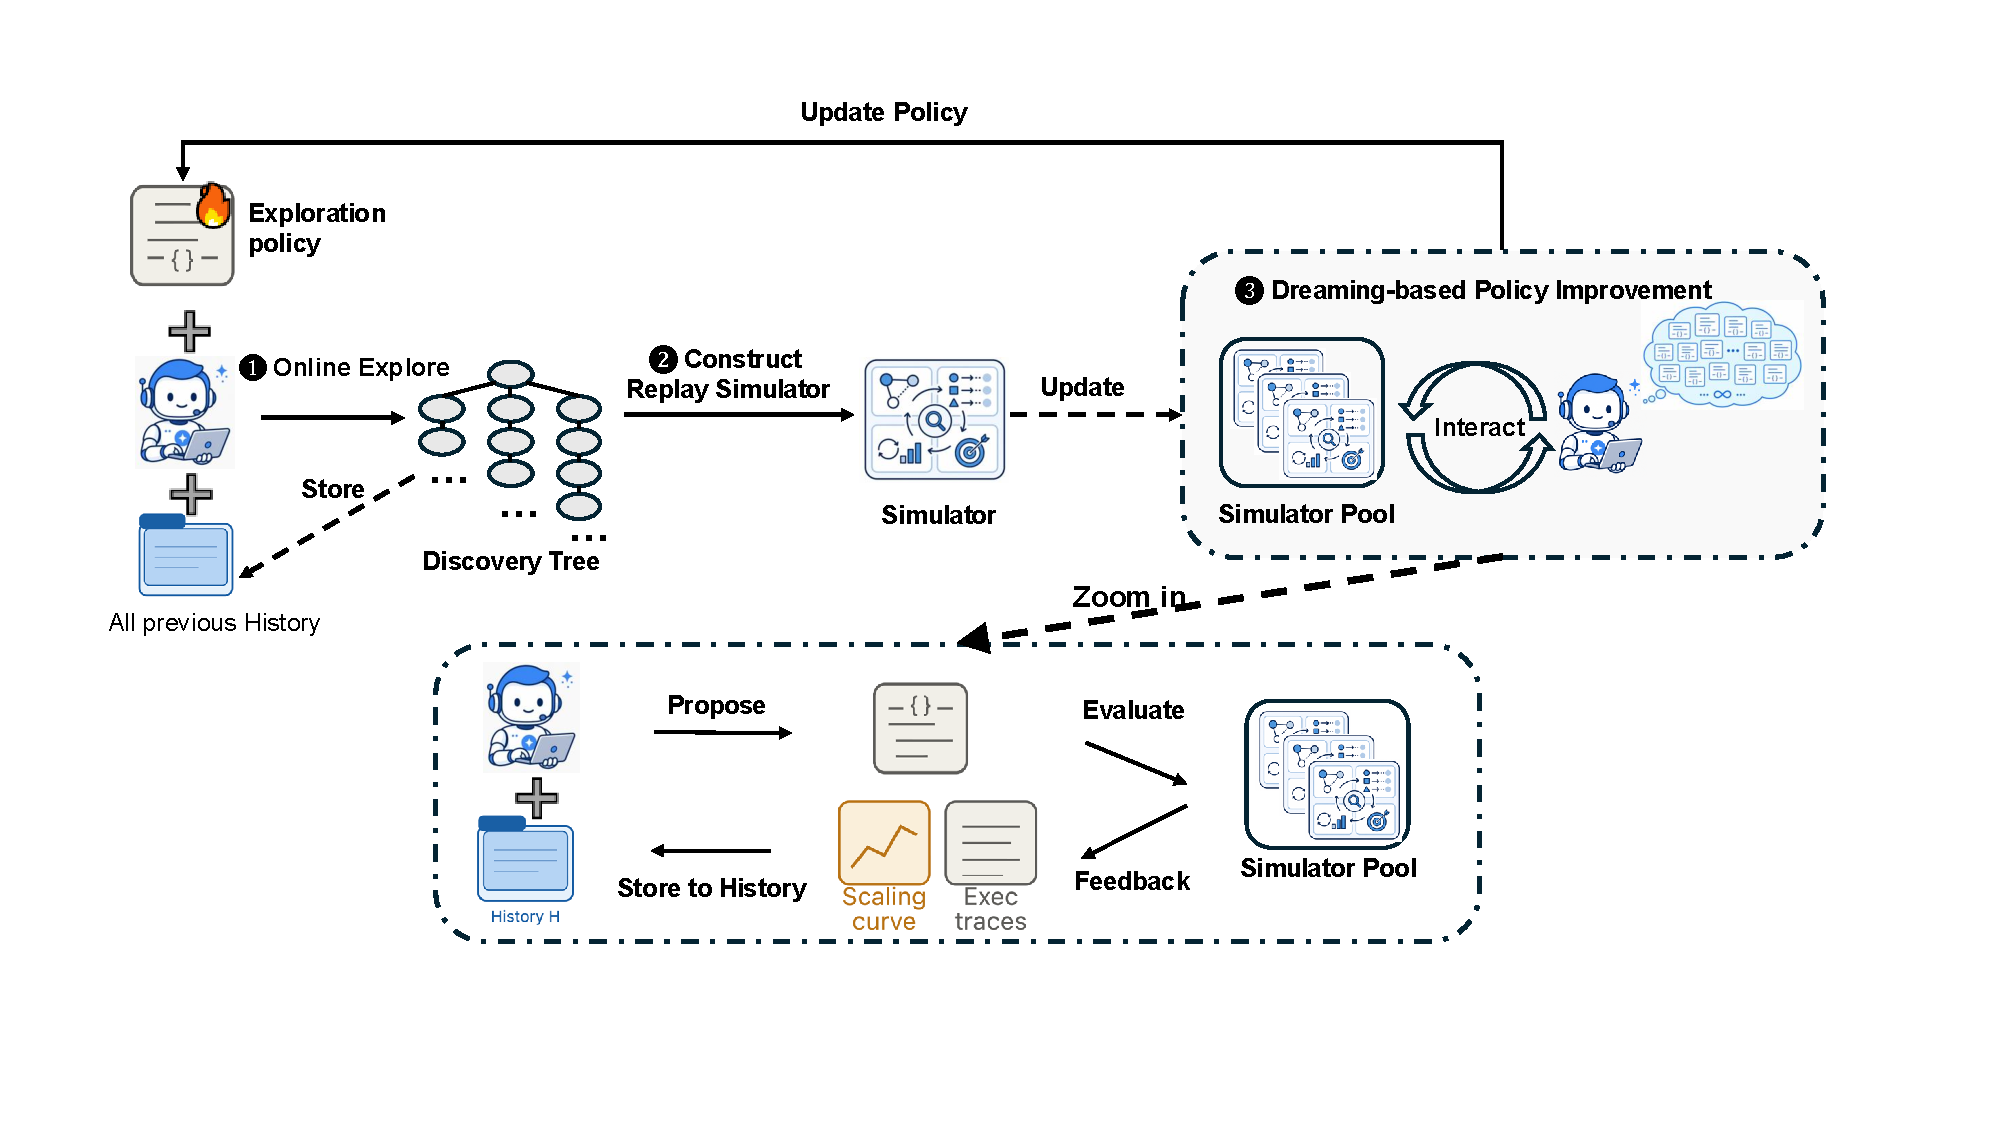
\includegraphics[width=0.93\linewidth]{Main_Text/Figures/Dream-RSI-latest.pdf}
    \caption{\textbf{Overview of \textsc{Dream-RSI}.} The system operates in a recursive self-improvement loop via three core stages: \textbf{\textcircled{1} Online Explore}, where the current exploration policy guides a coding agent to expand a discovery tree and log historical traces; \textbf{\textcircled{2} Construct Replay Simulator}, where the generated discovery tree is converted into a reusable simulator pool; and \textbf{\textcircled{3} Dreaming-based Policy Improvement}, where the agent "dreams" up a massive pool of alternative policies in its mind. It then feeds these candidate policies into the replay simulator to simulate executions and derive rapid feedback, continuously refining its strategy (detailed in the Zoom-in box). The updated policy then redeploys for the next round of online exploration.}
    \label{fig:method}
\end{figure}


Recursive self-improvement (RSI) has emerged as an ambitious goal for autonomous AI systems~\citep{202608.0051}. A common mechanism underlying RSI is an iterative discovery loop wherein agents generate candidate solutions, evaluate outcomes, incorporate feedback, and refine future iterations. Such discovery loops have driven substantial progress across scientific and algorithmic domains, including algorithm design~\citep{novikov2025alphaevolve,romera2024mathematical}, open-ended mathematical optimization~\citep{georgiev2025mathematical,anthropic2026riemann}, systems design~\citep{jaber2026autokernel,cao2026k}, and agent self-improvement~\citep{zhang2026darwin,zhang2026hyperagents,lee2026meta,zheng2026llms}, with these discoveries increasingly feeding into the development of more capable AI systems. As agent capabilities improve and self-improvement targets become challenging, discovery increasingly requires long-horizon exploration over vast search spaces, often spanning thousands of proposal--evaluation cycles~\citep{ye2026evaluation,openai2026navierstokes}. At this scale, the ability to orchestrate exploration becomes critical~\citep{zheng2026parallel}. Poor exploration can waste substantial computation and time, severely limiting the efficiency and scalability of RSI.

Existing approaches have largely relied on manually designed exploration strategies that remain largely fixed throughout discovery~\citep{novikov2025alphaevolve,yan2026pacevolve,du2026mlevolve,jiang2026deltaevolve,ye2026evaluation}. Fixed strategies cannot improve from accumulated discovery experience and may repeatedly allocate computation to ineffective search directions.  Recent work therefore seeks to optimize exploration policies online during discovery~\citep{liu2026evox}, but doing so faces two fundamental bottlenecks. First, feedback is delayed and expensive at the meta level: unlike evaluating an individual candidate, assessing an exploration policy requires observing how it shapes the subsequent discovery process over many proposal--evaluation cycles. Second, the meta-policy space is vast: a newly proposed policy may perform poorly, so many alternatives may need to be tried. Together, these challenges make meta-level improvement particularly costly: each policy may require a long online rollout before receiving useful feedback, making it difficult to efficiently close the self-improvement loop at the exploration layer. 

To address these bottlenecks, our key intuition is simple: a fast and inexpensive simulator of discovery would allow many exploration policies to be evaluated before costly online deployment. \textbf{Surprisingly, completed discovery histories already provide such a simulator.} While prior work treats past discovery history merely as static textual context~\citep{hu2025memory,ouyang2026reasoningbank} or training data for weight fine-tuning~\citep{yuksekgonul2026learning,wang2025thetaevolve}, a completed discovery process inherently records a structured tree of past exploration decisions and their realized code-execution outcomes. Drawing an analogy to model-based reinforcement learning and World Models~\citep{ha2018world,hafner2023mastering} (\S\ref{sec:history_environment}), once organized into a discovery tree, this history can serve as a \textbf{replay simulator}~\footnote{We use the terms replay simulator and worlds interchangeably.}. As illustrated in Figure~\ref{fig:motivation}, an alternative exploration strategy can navigate this pre-recorded tree to traverse different subsets of recorded branches, in different orders, with different parallel groupings and stopping decisions. Because all execution outcomes are already saved in the tree, evaluating a new strategy requires only reading past records without rerunning the underlying discovery agent or evaluator. This transforms meta-policy improvement from an expensive online trial-and-error process into a fast, simulation-based ``dreaming'' procedure.

Building on this insight, we introduce \textsc{Dream-RSI}, a framework for scalable and recursively self-improving meta-exploration in agent-driven discovery. We first make exploration explicit and programmable through a lightweight orchestration layer that controls branching, parallel exploration, and stopping while leaving the underlying coding agent unchanged. Rather than keeping this policy fixed, \textsc{Dream-RSI} establishes a closed-loop self-improvement mechanism across three core stages (Figure~\ref{fig:method}): \textbf{(1) Online Exploration}, where the current policy guides real-world discovery and logs historical execution traces; \textbf{(2) Simulator Construction}, where recorded discovery trees are converted into a reusable replay simulator pool; and \textbf{(3) Dreaming-based Policy Improvement}, where candidate policies are evaluated via low-cost "dreaming" over the simulator. The updated policy is then redeployed online to generate new discovery experience and expand the simulator pool, closing a RSI loop at the meta-exploration layer.

Empirically, we evaluate \textsc{Dream-RSI} across 8 scientific discovery tasks spanning three distinct domains: algorithm engineering, mathematical optimization, and GPU kernel engineering. In algorithm engineering (Lasso path solver), \textsc{Dream-RSI} outperforms standard libraries like \texttt{sklearn} and strong baselines while reducing agent calls by up to $162\times$ over \textsc{SimpleTES} and $1.7\times$ over fixed-exploration baselines. In mathematical optimization (sum-difference, autocorrelation, circle packing), it matches or surpasses strong baselines within $1\text{k}$ generations, yielding over $50\times$ budget savings compared to \textsc{SimpleTES}. In GPU kernel engineering (KernelBench), it either reaches target execution speeds using $1.79\times$--$2.43\times$ fewer generations or improves kernel performance by up to $2.09\times$ under identical budget constraints.  

In summary, our main contributions are as follows: 1) \textbf{History as Replay Simulator:} We conceptualize completed discovery histories as replay simulators. This makes delayed exploration feedback reusable for efficient meta-exploration policy evaluation.;   2) \textbf{Meta-Layer RSI Loop (\textsc{Dream-RSI}):} We introduce \textsc{Dream-RSI}, establishing a recursive self-improvement loop that continuously collects discovery histories through online exploration, constructs replay simulators from history to refine meta-exploration strategies via  dreaming, and redeploys the upgraded policy online; 3) \textbf{Empirical Validation:} We conduct experiments to demonstrate that \textsc{Dream-RSI} improves both discovery effectiveness and efficiency in several settings.


\begin{figure}
    \centering
    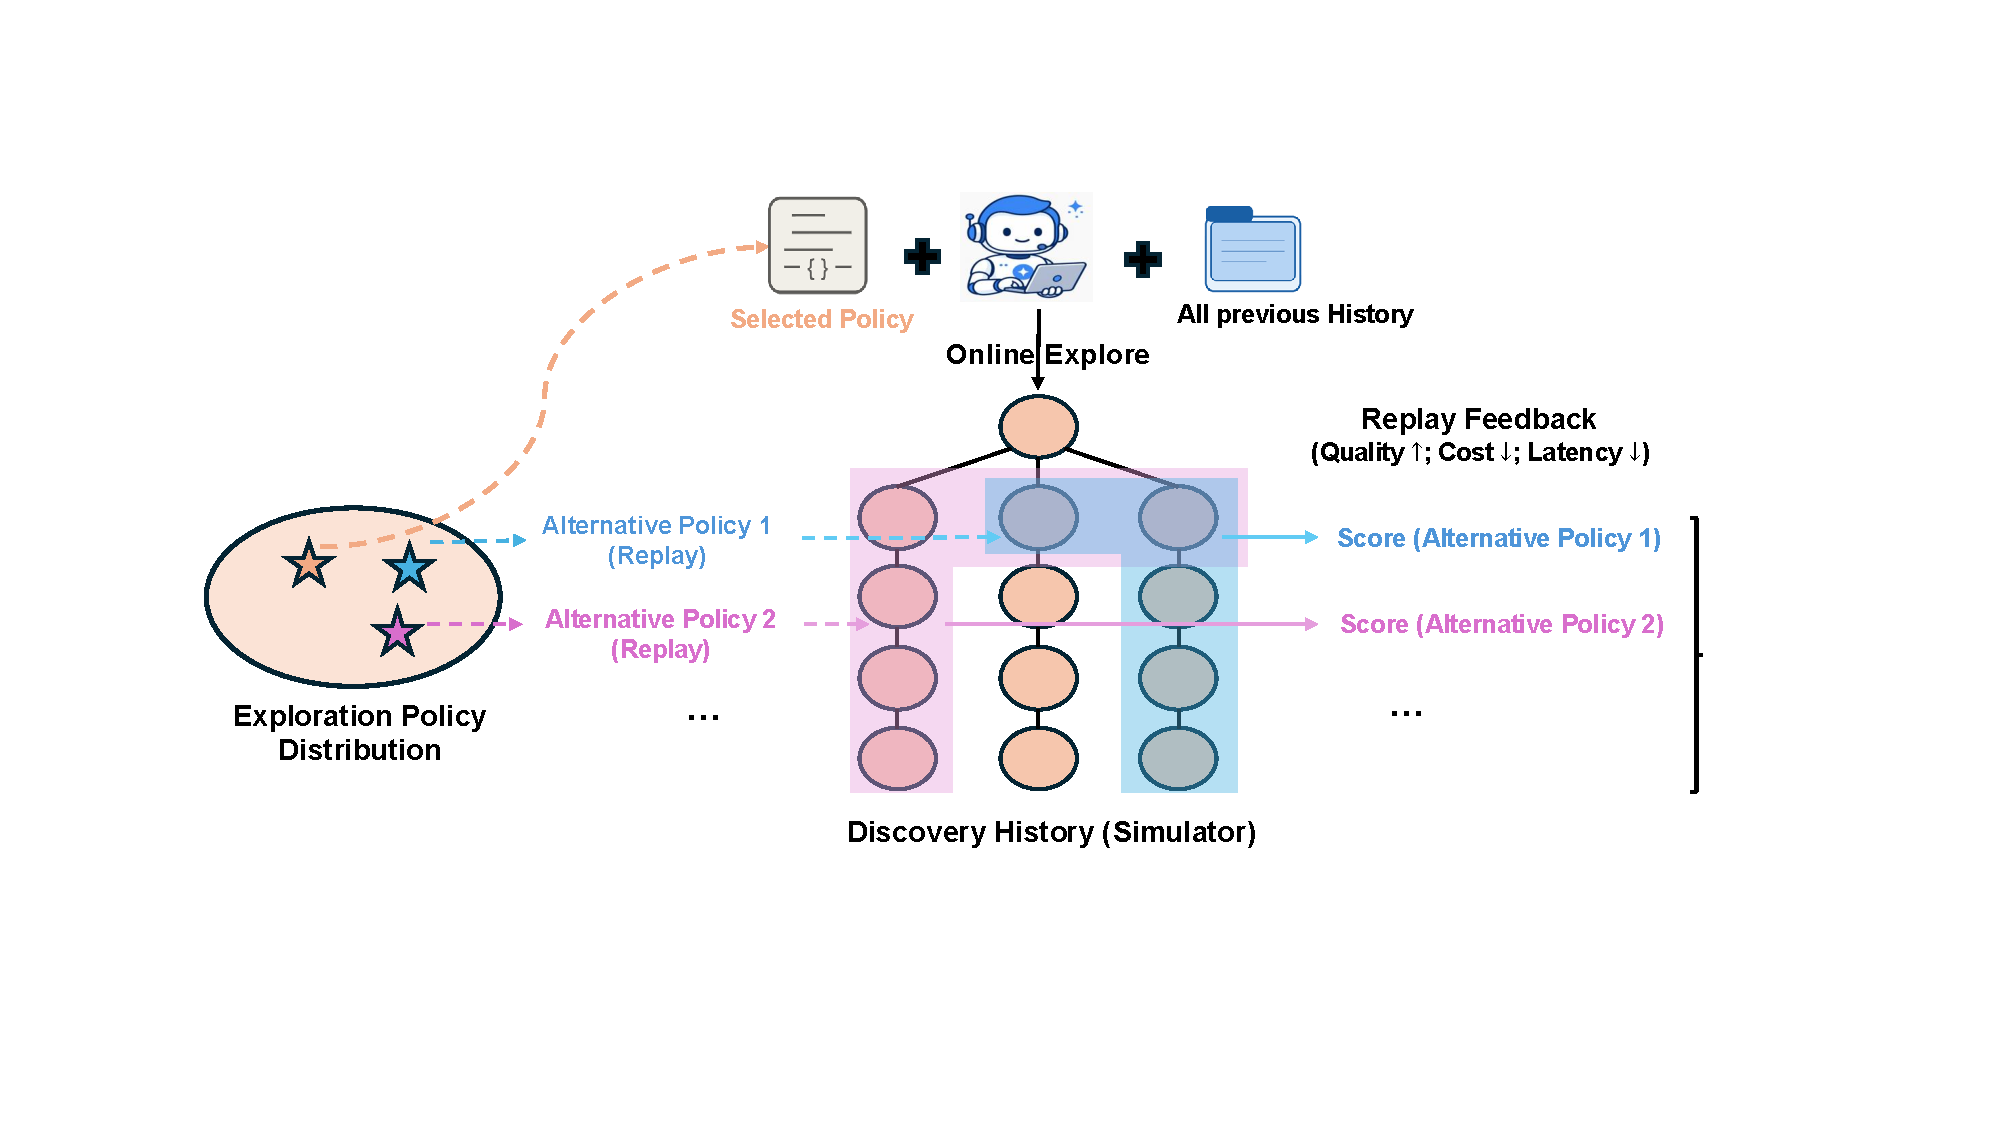
\includegraphics[width=0.92\linewidth]{Main_Text/Figures/HRS-latest.pdf}
    \caption{\textbf{Discovery history as a replay simulator.} A deployed policy first explores online to generate a structured discovery tree containing historical execution traces (each node denote an attempt with its full observation). Thousands of candidate policies can then be tested within this simulator—evaluating alternative choices of search branches, exploration orders, concurrency levels, and stopping rules. \textbf{Since all node outcomes are pre-stored, a single costly online run enables thousands of rapid, zero-execution-cost off-policy evaluations. This enables policy improvement through historical replay: the agent can “dream” over many alternative exploration strategies before redeploying the improved policy online.}}
    \label{fig:motivation}
\end{figure}

\section{Motivation: Discovery History as a Replay Simulator}
% \section{Motivation: Discovery History as a Replayable Environment}
\label{sec:history_environment}

Consider an agent navigating toward a goal in an unfamiliar environment. During its first traversal, the agent may follow inefficient routes, encounter
dead ends, backtrack, and gradually construct a map of the surrounding space. Once recorded, however, this experience becomes reusable: the resulting map
supports planning without requiring the agent to physically revisit every location. A new navigation policy can instead reason over the accumulated map,
avoid known dead ends, reconsider earlier decisions, and compare alternative
routes before acting~\citep{gupta2017cognitive}.

This idea parallels model-based reinforcement learning \citep{SUTTON1990216, m2023model}. A model captures how an environment evolves in response to an agent's actions, allowing policies to be trained or evaluated through simulated experience rather than
repeated interaction with the real environment~\citep{ha2018world}. The Dreamer family~\citep{hafner2019dream, hafner2020mastering, hafner2023mastering, hafner2025training} demonstrates this principle particularly clearly: an agent learns a compact dynamics model from collected experience and improves its policy by imagining trajectories within that model.

Long-horizon discovery admits an analogous structure. An exploration policy decides which directions to pursue, which candidates to refine, which branches to explore in parallel, and when to terminate. Executing the policy online produces a structured discovery history containing the explored branches, decision points, computational costs, and realized outcomes. As illustrated in
Figure~\ref{fig:motivation}, this history can subsequently be treated as an \emph{empirical replay simulator}: a grounded model of the portion of the discovery space that has already been observed.

Within this replay simulator, alternative exploration policies induce different trajectories through the recorded discovery tree. A policy may select a different subset of branches, prioritize them in a different order, issue different requests in parallel, or stop at an earlier point. Evaluating such a trajectory requires only revealing the outcomes already stored along the
selected branches, rather than rerunning the underlying coding agent and evaluator. Consequently, a single expensive online discovery run can support many inexpensive evaluations of alternative exploration strategies.


% Requires: \usepackage{amsmath,amssymb}


\section{\textsc{Dream-RSI}: Recursive Self-Improvement through Evolving Worlds}
\label{sec:replay-based-controller-improvement}


As shown in Figure~\ref{fig:method}, \textsc{Dream-RSI} alternates
between online exploration and offline ``dreaming'' to improve an
executable \emph{exploration policy} that allocates discovery computation.
During the online phase, the policy guides a fixed \emph{discovery agent}, while a fixed
\emph{evaluator} scores the resulting candidates and provides diagnostic
feedback. The resulting \emph{discovery tree} serves as a \emph{replay
world} in which alternative policies can be evaluated using recorded
outcomes. A fixed LLM-based \emph{policy-development agent} uses this
feedback to revise the \emph{exploration policy} code, and the best evaluated version is
deployed for the next online rollout. Only the exploration-policy code
changes; the underlying models, evaluator, and execution interfaces
remain fixed.

\paragraph{Discovery trees and the shared decision interface.}
A discovery tree is rooted at \(r\), which represents the initial
workspace state. Each non-root node \(v\) has exactly one
\emph{primary parent}, either the root or a previously created node.
This parent identifies where the attempt in \(v\) begins:
the discovery agent resumes the parent's saved workspace and uses
its accumulated observations as context to produce a new attempt. Node \(v\) preserves this
inherited history and records the outcome of the new
generation--evaluation attempt, including the resulting filesystem
snapshot, generated artifact, evaluation diagnostics, and score \(s_v\).
Scores follow a fixed task-scoring protocol, with larger values
indicating better quality.

In both online execution and offline replay, the exploration policy
observes a tree \(\mathcal T\), initially containing only the root,
and selects the nodes from which to continue exploration.
The eligible nodes form the set
\(A(\mathcal T)=\{r\}\cup\{v\in\mathcal T:v\text{ is a leaf}\}\),
where leaves are determined from the currently observed tree.
Let \(W\geq 1\) be the number of parallel workers, each of which can
execute one generation--evaluation request at a time (e.g. concurrent API calls).
The exploration policy's action is a batch \(C\in A(\mathcal T;W)\), where
\(A(\mathcal T;W)=\{C\subseteq A(\mathcal T):|C|\leq W\}\) is the feasible batch set.
Each selected node specifies the starting point of one attempt,
so the batch determines both where exploration continues and
how many attempts are scheduled in parallel. Both the online and offline phases use this same decision interface but differ in the
transition that follows a selected batch.

\paragraph{Online rollout.}
Let \(t=1,2,\ldots\) index the outer iterations, starting from an
initial policy \(\pi_1\) and an empty history \(\mathcal H_0=()\).
At iteration \(t\), policy \(\pi_t\) guides a new online rollout
with access to the completed discovery history \(\mathcal H_{t-1}\).
This history provides context for exploration but remains separate
from the new tree being constructed. The policy code stays fixed
throughout the rollout.

Let \(\mathcal T_{t}^k\) denote the new discovery tree after \(k\)
completed decision rounds, with \(\mathcal T_{t}^0=\{r\}\).
The rollout allows at most \(K_1\) rounds. At round $k \le K_1$, the \emph{exploration policy} chooses a node batch \(C_{t}^k \in A(\mathcal T_{t}^k;W)\) and each node \(v\in C_{t}^k\) is assigned to a worker.
The discovery agent uses \(v\)'s saved workspace and available
context to produce a new candidate, and the evaluator assesses
the result. These attempts run in parallel, each producing one
new child of its selected parent. Attaching the completed children
to the current tree yields \(\mathcal T_{t}^{k+1}\), while all
previously recorded nodes remain unchanged. This transition is stochastic because the discovery agent may
generate different outcomes from the same starting workspace. For the next round, the newly created
child becomes the selectable leaf of an extended branch, while the root remains selectable for opening further branches. The rollout ends when the policy selects an empty batch or completes \(K_1\) decision rounds. After the rollout terminates, its final tree is recorded as
\(\mathcal T_t\) and appended to the history, giving
\(\mathcal H_t= \mathcal H_{t-1} \cup \{\mathcal{T}_t\}\).
The method then enters the offline phase using this expanded collection of replay worlds.

\paragraph{Offline evaluation.}
During the offline phase of outer iteration \(t\), the history
\(\mathcal H_t\) remains fixed while the method constructs and
evaluates \(M\geq 1\) policy versions
\(\pi_t^0,\ldots,\pi_t^{M-1}\), starting with
\(\pi_t^0=\pi_t\).
Each version is evaluated separately on every historical tree
\(\mathcal T_i\), \(i=1,\ldots,t\), before the next version is
developed from the resulting feedback.
We use \(m\) to index policy versions, \(i\) to index replay worlds, and \(k\) to count decision rounds within one policy--world
evaluation. The outer index \(t\) is fixed throughout this phase
and is suppressed in the notation for replay trajectories and scores.


For each policy--tree pair \((m,i)\), replay resets the policy's
per-rollout state and starts from \(\mathcal T_i^{m,0}=\{r\}\).
Here, \(\mathcal T_i^{m,k}\subseteq\mathcal T_i\) denotes the subtree
revealed after \(k\) completed rounds. The full recorded tree
\(\mathcal T_i\) remains fixed; only the portion observed by the
policy evolves. At each decision, \(\pi_t^m\) selects a batch
\(C_i^{m,k}\in A(\mathcal T_i^{m,k};W)\) using the revealed
observations. Unlike online execution, replay returns recorded children of the
selected nodes deterministically rather than generating new candidates.
After the \emph{exploration policy} takes a nonempty batch $C_i^{m,k}$, the next observed tree is
\(\mathcal T_i^{m,k+1}
=\mathcal T_i^{m,k}
\cup\bigcup_{v\in C_i^{m,k}}
\operatorname{Child}(v;\mathcal T_i,\mathcal T_i^{m,k})\) where \(\operatorname{Child}(v;\mathcal T_i,\mathcal T_i^{m,k})\) denotes the node set containing unobserved children of $v$ on tree $\mathcal T_i$ given the current observed tree $T_i^{m,k}$. For \(v\ne r\), \(\operatorname{Child}(v;\mathcal T_i,\mathcal T_i^{m,k})\) is \(v\)'s unique recorded child, if one exists. Since \(v\) is a leaf of \(\mathcal T_i^{m,k}\), that child is still unrevealed.
For \(v=r\), replay returns the earliest-created child of \(r\)
outside \(\mathcal T_i^{m,k}\), opening one previously unrevealed branch.
In either case, \(\operatorname{Child}(v;\mathcal T_i,\mathcal T_i^{m,k})
=\emptyset\) when no recorded continuation remains. The newly revealed nodes expose their stored observations before
the policy makes its next decision.

Replay allows at most \(K_2\) decision rounds where each nonempty batch counts as one round, and terminates when
the policy selects \(C_i^{m,k}=\emptyset\), the round limit
\(k=K_2\) is reached, or \(\mathcal T_i^{m,k}=\mathcal T_i\),
meaning that all recorded nodes have been revealed.
Let \(k_i^{m,\star}\in\{0,\ldots,K_2\}\) denote the number of
completed rounds at termination, yielding the final subtree
\(\mathcal T_i^{m,k_i^{m,\star}}\subseteq\mathcal T_i\).

Thus, replay evaluates how far to pursue each opened branch,
how to group attempts into parallel batches, and when to open
another branch or stop. These decisions may differ across policies,
but each branch is traversed in its recorded parent--child order,
and no outcomes beyond \(\mathcal T_i\) are generated.




\paragraph{Replay objective.}
The replay objective balances discovery quality, execution cost,
and parallelism. Let
\(N_i^m=|\mathcal T_i^{m,k_i^{m,\star}}|-1\)
be the number of revealed non-root nodes.
Although replay itself does not execute new discovery attempts,
\(N_i^m\) counts the generation--evaluation requests represented
by its trajectory.
For fixed coefficients \(\beta_1,\beta_2\geq 0\), the replay score is
\begin{equation}
    V_i^m
    =
    \underbrace{
        \max_{v\in\mathcal T_i^{m,k_i^{m,\star}}} s_v
    }_{\text{discovery quality}}
    -
    \underbrace{
        \beta_1 N_i^m
    }_{\text{execution cost}}
    +
    \underbrace{
        \beta_2
        \frac{N_i^m}{\max\{1,k_i^{m,\star}\}}
    }_{\text{parallelism bonus}}.
    \label{eq:dream-rsi-replay-score}
\end{equation}
The first term measures the best solution quality attained during
replay. The second penalizes the
number of attempted generations. For a nonempty replay, the third
rewards the average number of attempts executed per decision round,
favoring policies that batch useful continuations rather than
execute them sequentially.

\paragraph{Policy improvement and selection.}
The evaluation score of policy version \(\pi_t^m\) is its average
replay score across the fixed history,
\(V^m=\frac{1}{t}\sum_{i=1}^{t}V_i^m\).
The offline phase begins by evaluating the current policy
\(\pi_t^0=\pi_t\).
For each \(m=0,\ldots,M-1\), the \emph{policy-development agent} examines
the replay trajectories and scores of \(\pi_t^m\), together with
feedback from earlier revisions, to identify successful decisions
and recurring failures. It then revises the executable policy code
to produce \(\pi_t^{m+1}\), which is evaluated on the same
\(t\) replay worlds.
Replay feedback is available to the development agent between
revisions.

After \(M\) revisions, the next online policy is selected from all
\(M\) evaluated versions as \(\pi_{t+1}=\pi_t^{m^\star}\), where
\(m^\star\in\operatorname*{arg\,max}_{m\in\{0,\ldots,M-1\}}V^m\).
Because the candidate set includes the current policy, this
selection satisfies \(V^{m^\star}\geq V^0\).
Thus, the selected policy $\pi_{t+1}$ is no worse than the current policy $\pi_t$
in average replay score on the fixed history \(\mathcal H_t\). The selected policy is then deployed online to collect
\(\mathcal T_{t+1}\), expanding the history available for the next offline improvement phase.



% \input{Main_Text/A more math-formal formulation}
% \section{History as Environment Driven Recursive Self-Improvement}
\label{sec:method}

We consider a scientific discovery process that iteratively generates and
evaluates candidate solutions. At each step, an \emph{exploration policy}
decides how search effort should be allocated---which directions to open, which
existing branches to refine, and when to prune or stop. Rather than fixing this
exploration policy throughout discovery, our goal is to improve the exploration process
itself from the experience it has already generated.

Our key idea is to transform accumulated exploration history into a
\emph{replayable environment} for learning exploration policy. After each
discovery cycle, we retain the complete evaluated exploration trace rather than
only the best solution. These traces expose the same state--action interface as
live discovery, allowing alternative controllers to make exploration decisions
and observe their historically realized consequences without rerunning the
underlying candidate-generation process. A controller-development agent then
proposes and improves executable controllers through interaction with these
historical environments. The selected controller is deployed in the next live
discovery cycle, whose resulting experience expands the environment for
subsequent improvement.

Formally, let $H_t$ denote all exploration experience accumulated through
discovery cycle $t$. Our recursive improvement loop is
\begin{equation}
    H_t
    \;\longrightarrow\;
    \mathcal{E}(H_t)
    \;\longrightarrow\;
    \pi_{t+1}
    \;\longrightarrow\;
    \tau_{t+1}
    \;\longrightarrow\;
    H_{t+1}=H_t\cup\{\tau_{t+1}\},
    \label{eq:outer-loop}
\end{equation}
where $\mathcal{E}(H_t)$ is the historical environment constructed from
accumulated traces, $\pi_{t+1}$ is the learned exploration controller, and
$\tau_{t+1}$ is the new trace generated by deploying it. The framework thus
consists of three stages: constructing a historical environment, improving
exploration controllers within that environment, and recursively deploying the
improved controller to generate new experience.


\subsection{Constructing the Historical Environment}
\label{sec:historical-environment}

\paragraph{Exploration history.}
Each discovery cycle explores a branching space of candidate solutions. A root
node opens a new search direction from the task seed, while subsequent nodes
refine previous attempts along the same branch. For every evaluated node, we
record its branch structure, parent, candidate artifact, evaluator score,
validity, failure information, and task-specific diagnostics. We denote the
observation associated with node $v$ by
\begin{equation}
    o_v =
    \bigl(
        b,d,s_v,z_v,
        \Delta_v^{\mathrm{seed}},
        \Delta_v^{\mathrm{parent}}
    \bigr),
\end{equation}
where $(b,d)$ identifies the branch and depth, $s_v$ is the evaluator score,
$z_v$ contains evaluation status and diagnostics, and the two deltas measure
progress relative to the cycle seed and the parent node. Failed attempts are
retained because they provide evidence about unsuccessful directions and
potentially recoverable errors.

A completed discovery cycle produces a frozen exploration trace
$\tau=(V,E,O)$ together with its execution metadata. Importantly, we preserve
the explored structure and intermediate outcomes rather than only the final
best candidate. The cumulative history
\begin{equation}
    H_t = \{\tau_1,\ldots,\tau_t\}
\end{equation}
therefore captures how discovery unfolded across previous cycles, including
successful trajectories, regressions, failures, and unexplored alternatives
within the recorded search structure.

\paragraph{From trace to environment.}
We turn these frozen traces into a stateful decision environment. At decision
step $k$, a controller observes only the revealed prefix
\begin{equation}
    P_k = \{(v,o_v): v \text{ has been probed}\}.
\end{equation}
Given $P_k$, the legal action set $\mathcal{A}(P_k)$ contains unopened roots and
the next unrevealed child of each opened branch whose parent has already been
revealed. The controller selects a batch
\begin{equation}
    B_k \subseteq \mathcal{A}(P_k),
    \qquad |B_k|\leq W,
\end{equation}
where $W$ is the available worker capacity. This interface captures both
sequential exploration decisions and parallel allocation of search effort.

The key design is that \emph{live discovery and historical replay share the
same controller interface}. In live mode, probing a node launches the
candidate-generation agent and evaluator and returns the resulting observation.
In replay mode, the identical action reveals the observation previously
recorded for that node. State construction, legal actions, controller inputs,
probe accounting, and parallel execution accounting are otherwise shared.
Consequently, a controller developed through replay is directly executable in
live discovery without conversion from a simulator-specific policy.

The historical environment is deliberately restricted to observed support.
Replay can test how a controller would select, order, batch, prune, or stop
among previously evaluated nodes, but it never predicts the outcome of a
candidate that was not generated in the original trace. We therefore reuse the
\emph{decision structure} and realized consequences of previous exploration
without fabricating counterfactual candidate outcomes.


\subsection{Improving Exploration Controllers}
\label{sec:controller-improvement}

\paragraph{Executable controllers.}
An exploration controller $\pi$ is an executable program that maps the
currently revealed exploration state to future search decisions:
\begin{equation}
    \pi:
    \bigl(P_k,\mathcal{A}(P_k)\bigr)
    \longrightarrow B_k .
\end{equation}
The controller operates at two resolutions. Before a discovery cycle, it
selects a structural exploration envelope
\begin{equation}
    g=(M,D),
\end{equation}
where $M$ determines the available search width and $D$ the maximum refinement
depth. Within that envelope, the controller adaptively decides which roots to
open, which branches to refine or recover, and when further exploration is no
longer worthwhile.

Controllers are constrained to be deterministic and prefix-only. They may use
observed branch trajectories, relative improvements, failure evidence, and
remaining legal search depth, but cannot access unrevealed outcomes, winning
node identities, or the final best score of a historical trace. These
restrictions ensure that replay exposes only information that would have been
available at the corresponding point in live discovery.

\paragraph{Agentic controller improvement.}
Given $H_t$, we instantiate the historical environment
$\mathcal{E}(H_t)$ and provide a controller-development agent with the
controller API, previous controller implementations, and feedback from earlier
proposal rounds. The agent iteratively proposes executable controller code,
evaluates it through replay, inspects its behavior, and revises the controller:
\begin{equation}
    \pi^{(j)}
    \xrightarrow{\;\mathcal{E}(H_t)\;}
    F^{(j)}
    \longrightarrow
    \pi^{(j+1)},
    \label{eq:controller-learning}
\end{equation}
where $F^{(j)}$ summarizes replay performance and decision-level execution
feedback. Such feedback exposes behaviors such as premature stopping,
over-pruning, excessive probing, poor recovery decisions, or insufficient use
of parallelism. The development agent can use these observations to modify the
controller implementation in subsequent proposal rounds.

This design separates the \emph{learner} from the \emph{learned object}: the
controller-development agent performs meta-level optimization, while the
resulting controller is a lightweight executable policy that governs live
exploration.

\paragraph{Replay objective.}
A useful exploration controller should recover strong outcomes while spending
as little search effort as possible. For historical trace $i$ and exploration
setting $\beta$, let $Q_{i,\beta}$ denote the number of probes selected by the
controller, $S_{i,\beta}$ its best revealed score, $G_i$ the best score
available anywhere in the trace, and $N_i$ the number of evaluated nodes.
We measure normalized attainment as
\begin{equation}
    a_{i,\beta}
    =
    \operatorname{clip}
    \left(
        \frac{S_{i,\beta}}{G_i},0,1
    \right).
\end{equation}
Here, $G_i$ is used only for offline evaluation and is never exposed to the
controller.

Sweeping a fixed set of exploration settings yields a probe--attainment
frontier for each trace. We summarize this frontier using its normalized area,
$\operatorname{AUC}_i(\pi)$, which rewards controllers that recover high-quality
historical outcomes without exhaustively probing the trace. Because probe
efficiency alone can favor highly sequential policies that are inefficient in
live discovery, we additionally penalize unnecessary sequential decision
rounds. The final controller objective is
\begin{equation}
    J(\pi)
    =
    \frac{1}{|\mathcal{T}|}
    \sum_{i\in\mathcal{T}}
    \operatorname{AUC}_i(\pi)
    -
    \lambda
    \frac{1}{|\mathcal{T}|}
    \sum_{i\in\mathcal{T}}
    P_i,
    \label{eq:controller-objective}
\end{equation}
where $P_i$ measures the controller's sequential-round cost relative to its
probe usage on trace $i$. We select the highest-scoring valid controller across
proposal rounds. Detailed definitions of the frontier metric, parallelism
penalty, and controller validation are provided in Appendix~\ref{app:controller}.


\subsection{Recursive Deployment}
\label{sec:recursive-deployment}

After controller development, the selected controller $\pi_{t+1}$ is deployed
directly in the next live discovery cycle through the same interface used
during historical replay. Its actions now launch real candidate-generation and
evaluation jobs rather than revealing stored outcomes. The resulting
exploration trace $\tau_{t+1}$---including successful candidates, failures,
branch trajectories, scores, and execution decisions---is frozen and appended
to the cumulative history:
\begin{equation}
    H_{t+1}
    =
    H_t \cup \{\tau_{t+1}\}.
\end{equation}

The enlarged history then defines a new historical environment
$\mathcal{E}(H_{t+1})$ for learning the next controller. Because the replay pool
is cumulative, later controllers are evaluated across environments generated
by multiple previous controllers rather than only the most recent trajectory.
Each deployed controller therefore changes the experience distribution from
which its successor is learned, closing the recursive loop
\begin{equation}
    H_t
    \rightarrow
    \mathcal{E}(H_t)
    \rightarrow
    \pi_{t+1}
    \rightarrow
    H_{t+1}
    \rightarrow
    \mathcal{E}(H_{t+1})
    \rightarrow
    \pi_{t+2}
    \rightarrow \cdots .
\end{equation}

In summary, \textbf{History as Environment} converts the by-product of
discovery into a reusable substrate for improving future discovery. Historical
exploration provides the environment, a controller-development agent learns
how search should be conducted within that environment, and live deployment
generates the experience from which the next exploration controller can be
improved.
\section{Experiments}
We evaluate \textsc{Dream-RSI} across three scientific discovery domains: algorithm engineering, kernel optimization and math optimization. Our primary controlled baseline is Recursive Fixed Exploration, which uses the same underlying discovery setting and initialization but keeps the exploration policy fixed across recursive discovery rounds. We additionally compare against task-specific domain baselines. 

Across all tasks, \textsc{Dream-RSI} and Recursive Fixed Exploration
use the same discovery agent, evaluator, initialization, and resource constraints.
Both methods start from the same manually designed exploration policy.
This exploration policy follows a simple \emph{parallel refining} strategy: it launches
multiple independent exploration workspaces in parallel, with each workspace
maintaining its own local discovery trajectory and repeatedly refining its
current candidate based on the history accumulated within that workspace.
The two methods therefore follow the same exploration policy in the first
discovery round. In subsequent rounds, while Recursive Fixed Exploration keeps its exploration policy static, \textsc{Dream-RSI} progressively refines the policy by dreaming over a replay simulator conditioned on accumulated global discovery history, subsequently deploying the updated policy in each new round. The discovery cost is quantified by the total cumulative number of discovery-agent calls.


Specifically, we evaluate Gemini-3.1 Pro and Gemini-3.7-Flash across multiple recursive discovery rounds via the Gemini CLI~\footnote{\url{https://geminicli.com/}}. Under Recursive Fixed Exploration, each round for Gemini-3.1 Pro executes 10 parallel workspaces with up to 11 refinement steps ($10 \times 11 = 110$ discovery-agent calls), whereas Gemini-3.7-Flash operates 32 parallel workspaces with up to 20 refinement steps ($32 \times 20 = 640$ calls). \textsc{Dream-RSI} maintains identical per-round budgets, aligning with the baseline in Round 1 while progressively updating its policy in subsequent rounds. Further details on recursive rounds, task setups, resource budgets, and evaluation protocols follow below.



\usepgfplotslibrary{groupplots}
\pgfplotsset{compat=1.18}

% ============================================================
% Scaling data
% Metric: arithmetic mean runtime over six real downstream tasks
% Lower is better.
% ============================================================

% ------------------------------------------------------------
% Gemini-3.1-Pro: Fixed Exploration
% ------------------------------------------------------------
\pgfplotstableread{
compute avg iter
110 5267.0500 1
220 5365.4000 2
330 5295.2333 3
440 4691.0833 4
550 3587.0667 5
}\probaseline

% ------------------------------------------------------------
% Gemini-3.1-Pro: Dream-RSI
% Iter 1 shares the same initialization
% ------------------------------------------------------------
\pgfplotstableread{
compute avg iter
110 5267.0500 1
119 5349.1500 2
147 5368.9000 3
234 5705.4333 4
317 2931.0000 5
}\proours

% ------------------------------------------------------------
% Gemini-3.7-Flash: Fixed Exploration
% Iter 1--2 have no downstream evaluation
% ------------------------------------------------------------
\pgfplotstableread{
compute avg iter
640  2735.6 1
1280 2988.3 2
1920 3011.1333 3
2560 2909.1833 4
3200 2516.6833 5
}\flashbaseline

% ------------------------------------------------------------
% Gemini-3.7-Flash: Dream-RSI
% Iter 1 has no downstream evaluation
% ------------------------------------------------------------
\pgfplotstableread{
compute avg iter
640  2735.6 1
976  2394.9167 2
1230 2378.0500 3
1529 2327.7000 4
1879 2350.5833 5
}\flashours


% ============================================================
% Main figure
% ============================================================

\begin{figure*}[t]
\centering

% ============================================================
% (a) Final performance table
% ============================================================

\resizebox{\textwidth}{!}{%
\begin{tabular}{l r r rr rrrr r}
\toprule

\textbf{Method}
& \textbf{Model}
& \textbf{Compute}
& \multicolumn{2}{c}{\textit{Non-biological}}
& \multicolumn{4}{c}{\textit{Biological}}
& \textbf{Avg.}
\\

\cmidrule(lr){4-5}
\cmidrule(lr){6-9}

&
&
&
\textbf{Gisette}
&
\textbf{RCV1}
&
\textbf{DNA}
&
\textbf{Leukemia}
&
\textbf{Colon}
&
\textbf{Duke Breast}
&
\\

\midrule

\multicolumn{10}{l}{\textit{Previous solvers}} \\[1pt]

sklearn
& --
& --
& 11275.2
& 252881.7
& 93.8
& 227.2
& 229.8
& 374.0
& 44180.3
\\

glmnet
& --
& --
& 9063.6
& 73072.8
& 351.9
& 45.0
& 24.2
& 47.7
& 13767.5
\\

SimpleTES
& gpt-oss-120b
& 51{,}200
& 3141.9
& 19625.6
& 15.9
& 15.5
& 11.6
& 18.1
& 3804.8
\\

SimpleTES $\dagger$
& gpt-oss-120b
& 51{,}200
& 8651.0
& 41143.1
& 37.6
& 28.2
& 19.5
& 31.1
& 8318.4
\\

\midrule

\multicolumn{10}{l}{\textit{Our System}} \\[1pt]

Recursive Fixed Exploration
& Gemini-3.1-Pro
& 550
& 1861.8
& 19550.1
& 41.5
& 26.1
& 14.5
& 28.4
& 3587.1
\\

&
Gemini-3.7-Flash
& 3200
& 1133.1
& 13873.0
& 29.8
& 24.1
& 15.7
& 24.4
& 2516.7
\\

\textbf{\textsc{Dream-RSI}}
& Gemini-3.1-Pro
& 317
& 2841.0
& 14616.0
& 49.9
& 30.2
& 16.4
& 32.5
& 2931.0
\\

&
Gemini-3.7-Flash
& 1879
& 1091.9
& 12923.4
& 31.4
& 21.0
& 12.2
& 23.6
& \textbf{2350.6}
\\

\bottomrule
\end{tabular}%
}

\vspace{0.08cm}

{\small\textbf{(a) Final performance.}}

\vspace{0.27cm}


% ============================================================
% (b) Scaling curves
% ============================================================

\begin{tikzpicture}

\begin{groupplot}[
group style={
  group size=2 by 1,
  horizontal sep=0.1\textwidth
},
width=0.5\textwidth,
height=4.85cm,
grid=major,
major grid style={
  gray!16,
  line width=0.3pt
},
axis line style={
  black!55,
  line width=0.65pt
},
tick style={
  black!55,
  line width=0.5pt
},
tick align=outside,
tick label style={
  font=\scriptsize,
  text=black!80
},
xlabel style={
  font=\small,
  yshift=1pt
},
ylabel style={
  font=\small
},
title style={
  font=\small\bfseries,
  yshift=2pt
},
scaled ticks=false,
clip=false
]


% ============================================================
% Left: Gemini-3.1-Pro
% ============================================================

\nextgroupplot[
title={Gemini-3.1-Pro},
xmin=50,
xmax=600,
ymin=2800,
ymax=6000,
xtick={100,300,500},
ytick={3000,4000,5000,6000},
xlabel={Discovery Compute},
ylabel={Avg. Runtime (ms)},
xticklabel style={
  /pgf/number format/fixed,
  /pgf/number format/precision=0
},
yticklabel style={
  /pgf/number format/fixed,
  /pgf/number format/precision=0,
  /pgf/number format/1000 sep={,}
},
legend to name=scalinglegend,
legend columns=2,
legend style={
  draw=none,
  font=\footnotesize,
  /tikz/every even column/.append style={
    column sep=1.4em
  }
}
]


% ------------------------------------------------------------
% Gemini-3.1-Pro: Fixed Exploration
% ------------------------------------------------------------

\addplot[
color=blue!75!black,
line width=1.7pt,
mark=square*,
mark size=2.5pt,
point meta=explicit symbolic,
nodes near coords,
every node near coord/.append style={
  font=\tiny,
  text=blue!75!black,
  anchor=north,
  yshift=-1.5pt,
  fill=white,
  fill opacity=0.90,
  text opacity=1,
  inner sep=0.7pt
}
]
table[
x=compute,
y=avg,
meta=iter
] {\probaseline};

\addlegendentry{Recursive Fixed Exploration}


% ------------------------------------------------------------
% Gemini-3.1-Pro: Dream-RSI
% ------------------------------------------------------------

\addplot[
color=red!80!black,
line width=1.9pt,
mark=*,
mark size=2.8pt,
point meta=explicit symbolic,
nodes near coords,
every node near coord/.append style={
  font=\tiny,
  text=red!80!black,
  anchor=south,
  yshift=1.5pt,
  fill=white,
  fill opacity=0.90,
  text opacity=1,
  inner sep=0.7pt
}
]
table[
x=compute,
y=avg,
meta=iter
] {\proours};

\addlegendentry{\textsc{Dream-RSI}}


% ============================================================
% Right: Gemini-3.7-Flash
% ============================================================

\nextgroupplot[
title={Gemini-3.7-Flash},
xmin=500,
xmax=3400,
ymin=2250,
ymax=3100,
xtick={1000,2000,3000},
ytick={2250,2500,2750,3000},
xlabel={Discovery Compute},
ylabel={},
xticklabel style={
  /pgf/number format/fixed,
  /pgf/number format/precision=0,
  /pgf/number format/1000 sep={,}
},
yticklabel style={
  /pgf/number format/fixed,
  /pgf/number format/precision=0,
  /pgf/number format/1000 sep={,}
}
]


% ------------------------------------------------------------
% Gemini-3.7-Flash: Fixed Exploration
% ------------------------------------------------------------

\addplot[
color=blue!75!black,
line width=1.7pt,
mark=square*,
mark size=2.5pt,
point meta=explicit symbolic,
nodes near coords,
every node near coord/.append style={
  font=\tiny,
  text=blue!75!black,
  anchor=south,
  yshift=1.5pt,
  fill=white,
  fill opacity=0.90,
  text opacity=1,
  inner sep=0.7pt
}
]
table[
x=compute,
y=avg,
meta=iter
] {\flashbaseline};


% ------------------------------------------------------------
% Gemini-3.7-Flash: Dream-RSI
% ------------------------------------------------------------

\addplot[
color=red!80!black,
line width=1.9pt,
mark=*,
mark size=2.8pt,
point meta=explicit symbolic,
nodes near coords,
every node near coord/.append style={
  font=\tiny,
  text=red!80!black,
  anchor=south,
  yshift=1.5pt,
  fill=white,
  fill opacity=0.90,
  text opacity=1,
  inner sep=0.7pt
}
]
table[
x=compute,
y=avg,
meta=iter
] {\flashours};


\end{groupplot}

\end{tikzpicture}


% ============================================================
% Shared legend
% ============================================================

\vspace{0.00cm}

{\centering
\pgfplotslegendfromname{scalinglegend}
\par
}

\vspace{0.015cm}

{\small\textbf{(b) Recursive Discovery Dynamics.}}

\vspace{-0.05cm}


% ============================================================
% Caption
% ============================================================

\caption{
\textbf{Lasso regularization-path discovery results.}
\textbf{(a)} Final wall-clock runtime on six held-out downstream tasks;
lower is better.
\textbf{Compute} denotes the cumulative number of discovery-agent calls.
\textbf{(b)} \textbf{Recursive discovery dynamics.} Average downstream runtime across six held-out tasks versus cumulative discovery compute for Gemini-3.1-Pro and Gemini-3.7-Flash. Numbers next to markers denote recursive rounds (iterations). Lower is better.
}

\label{fig:lasso-main}

\end{figure*}


\subsection{Algorithm Engineering}
\label{subsec:lasso}

In this task, we consider \textbf{Lasso Regularization Path} as our algorithm-engineering task, a fundamental computational primitive in high-dimensional statistics that is widely used in model selection and cross-validation across domains such as genomics and finance. We follow the benchmark setting of SimpleTES~\citep{ye2026evaluation}, where the goal is to discover efficient implementations of the complete Lasso regularization path while preserving numerical correctness. During discovery, we use the same 17 synthetic instances as SimpleTES, which cover diverse problem regimes in terms of dimensionality, sparsity, feature correlation, and active-set structure. To evaluate whether the discovered algorithms generalize beyond the search distribution, we additionally evaluate them on six held-out downstream datasets spanning both biological and non-biological domains. 

\paragraph{Baselines and Setup.}
We compare against standard Lasso solvers
\textbf{sklearn}~\citep{pedregosa2011scikit} and
\textbf{glmnet}~\citep{friedman2010regularization},
as well as \textbf{SimpleTES}~\citep{ye2026evaluation}, which uses
GPT-OSS-120B with a reported budget of 51,200 generations.
We additionally include Recursive Fixed Exploration as our controlled baseline. Specifically, we run both Recursive Fixed Exploration and \textsc{Dream-RSI} for 5 rounds.

\paragraph{Main Results.}
Figure~\ref{fig:lasso-main}(a) summarizes the Lasso discovery results.
Across both discovery-agent backbones, \textsc{Dream-RSI} achieves a better
downstream quality--compute trade-off than Recursive Fixed Exploration.
With Gemini-3.1 Pro, it reduces the average runtime across the six held-out
datasets from 3587.1\,ms to 2931.0\,ms while using only 317 discovery-agent
calls, compared with 550 calls for fixed exploration.
With Gemini-3.7-Flash, \textsc{Dream-RSI} further reduces the average runtime
from 2516.7\,ms to 2350.6\,ms using 1879 calls instead of 3200. Despite using substantially less discovery compute, the resulting solvers also
outperform the standard sklearn and glmnet implementations on all six held-out
datasets. Compared with SimpleTES, which uses 51,200 generations,
\textsc{Dream-RSI} achieves lower average downstream runtime with roughly
two orders of magnitude fewer discovery-agent calls. Notably, the program discovered by Gemini-3.1-Pro appears particularly well suited to large-scale matrices such as RCV1. In contrast, Gemini-3.7-Flash discovers a more general-purpose program that performs consistently across different problem scales.

\paragraph{Recursive Discovery Dynamics.}
Figure~\ref{fig:lasso-main}(b) illustrates the trajectory of downstream performance across recursive discovery rounds relative to cumulative discovery compute. By design, both methods share identical search behavior in the initial round. In subsequent rounds, Recursive Fixed Exploration maintains a static exploration policy, whereas \textsc{Dream-RSI} progressively refines and redeploys its policy via dreaming over accumulated discovery history. Consequently, the two trajectories diverge markedly: \textsc{Dream-RSI} consistently achieves superior downstream performance while requiring substantially lower cumulative compute across both Gemini-3.1-Pro and Gemini-3.7-Flash.


\paragraph{Discovered Solver Analysis.}
We further analyze the discovered solver, with its implementation provided in
the Appendix \ref{app:discovered-lasso}. Unlike SimpleTES, which switches between LARS and coordinate
descent according to problem dimensions, the discovered solver introduces
adaptivity within the active-set optimization itself. It combines strong-rule
screening with Cauchy--Schwarz-based KKT pruning, selectively recomputing exact
gradients only when the bound cannot certify a feature and falling back to a
full refresh when pruning becomes ineffective. This adaptive verification
scheme is further integrated with efficient active-set bookkeeping, lazy
Gram-matrix construction, and hardware-aware implementation.


\begin{table}[t!]
\centering
\caption{
Performance comparison on mathematical discovery tasks.
Higher is better for \textbf{Sum Diff} and \textbf{Circle Packing}, while lower is better for \textbf{Auto Correlation}.
Best results are shown in \textbf{bold}.
}
\label{tab:downstream_results}
\small
\setlength{\tabcolsep}{1pt}
\renewcommand{\arraystretch}{1.15}
\vspace{0.1in}
\begin{tabular}{llccc}
\toprule
\textbf{Method}
& \textbf{LLM}
& \textbf{Sum Diff ($\uparrow$)}
& \textbf{Auto Correlation ($\downarrow$)}
& \textbf{Circle Packing ($\uparrow$)} \\
\midrule

AlphaEvolve
& Gemini-2.0 Pro + Flash 
& -- &  1.455700 &  2.635862 \\

AlphaEvolveV2
& Gemini-2.0 Pro + Flash 
& 1.121936 & -- & \textbf{2.635983} \\

OpenEvolve 
& - 
& -- &  1.460000 &  - \\

CodeEvolve 
& -
& -- & -- & 2.635980 \\

ShinkaEvolve 
& Mixed 
& -- &  1.457800 &  2.635982 \\

TTS-Discovery
& Qwen3-8B 
& -- & -- &  \textbf{2.635983} \\

ThetaEvolve
& Distilled-Qwen3-8B 
& -- & 1.493000 & \textbf{2.635983} \\

EvoX
& Gemini-3.0-Pro 
& -- & 1.458900 & 2.635900 \\

SimpleTES
& GPT-OSS-120B 
& 1.143975 & \bf 1.453675 & \textbf{2.635983} \\


\midrule
\textit{Our System} \\
Recursive Fixed Exploration
& Gemini-3.1-Pro 
& 1.144047 & 1.456001 & \textbf{2.635983} \\

\textsc{Dream-RSI}
& Gemini-3.1-Pro  
& \textbf{1.145427}
& 1.456375
& \textbf{2.635983} \\

\bottomrule
\end{tabular}
\end{table}



\subsection{Mathematics Optimization}

We further evaluate \textsc{Dream-RSI} on three mathematical discovery tasks spanning discrete combinatorial optimization, geometric optimization, and functional optimization: the \textbf{Sum--Difference Problem}, \textbf{Circle Packing}, and \textbf{Autocorrelation Inequalities}. The goal of these problems is to discover high-quality solutions that optimize task-specific mathematical objectives under their respective constraints. Formal definitions of the three tasks are provided in Appendix.

We use Gemini-3.1 Pro via the Gemini CLI as the discovery agent for both Recursive Fixed Exploration and \textsc{Dream-RSI} for 10 rounds. For each task, the agent iteratively proposes and evaluates candidate constructions or optimization procedures according to the task-specific objective. We compare against a broad set of existing automated discovery systems, including AlphaEvolve~\citep{novikov2025alphaevolve}, AlphaEvolveV2~\citep{georgiev2025mathematical}, OpenEvolve~\citep{openevolve}, CodeEvolve~\citep{assumpccao2025codeevolve}, ShinkaEvolve~\citep{lange2026shinkaevolve}, TTS-Discovery~\citep{yuksekgonul2026learning}, ThetaEvolve~\citep{wang2025thetaevolve}, EvoX~\citep{liu2026evox}, and SimpleTES~\citep{ye2026evaluation}.

\paragraph{Results.}
Table~\ref{tab:downstream_results} summarizes the results across the three mathematical discovery tasks.
\textsc{Dream-RSI} achieves a Sum--Difference score of $1.145427$, outperforming SimpleTES and Recursive Fixed Exploration.
On Circle Packing, it reaches $2.635983$, matching the strongest reported result among the compared methods.
For Autocorrelation, \textsc{Dream-RSI} obtains $1.456375$, remaining competitive with existing discovery systems. Notably, SimpleTES achieves state-of-the-art performance on Autocorrelation Inequalities, but requires 51,200 generations, significantly more than the fewer than 1,000 generations used by our approach.
Overall, these results show that our \textsc{Dream-RSI} generalize well on mathematics optimization.



\begin{figure}[t]
    \centering
    \definecolor{oursblue}{HTML}{0072B2}
\definecolor{baselinegray}{HTML}{6B7280}
\usepgfplotslibrary{groupplots}
\begin{tikzpicture}

\begin{groupplot}[
  group style={group size=2 by 2,horizontal sep=1.00cm,vertical sep=1.45cm},
  width=7.3cm,
  height=4.4cm,
  xmin=0,
  axis lines=left,
  axis line style={black!55,line width=0.65pt},
  xmajorgrids=false,
  ymajorgrids=true,
  grid style={black!8,line width=0.30pt},
  scaled ticks=false,
  tick align=outside,
  tick style={black!55,line width=0.50pt},
  tick label style={font=\scriptsize,text=black!80},
  title style={font=\small\bfseries,yshift=3pt},
  xlabel style={font=\small,yshift=2pt},
  ylabel style={font=\small},
  clip=true,
  clip marker paths=true,
  restrict x to domain=1:2000,
  unbounded coords=discard,
  filter discard warning=false
]

% ============================================================
% VGG16
% ============================================================

\nextgroupplot[
  title={VGG16},
  xmax=1050,
  ymin=0.35,
  ymax=0.57,
  xtick={0,250,500,750,1000},
  xticklabels=\empty,
  ytick={0.35,0.40,0.45,0.50,0.55},
  ylabel={Performance ($1/\mathrm{ms}$)},
  legend to name=sharedlegend,
  legend columns=2,
  legend style={draw=none,font=\small,column sep=1.4em}
]

\addplot[
  const plot,
  color=oursblue,
  line width=2.55pt,
  mark=*,
  mark size=1.35pt,
  mark options={fill=oursblue,draw=oursblue}
]
table[x=budget,y=score]
{Main_Text/raw_data/data/vgg16_ours.dat};

\addlegendentry{\textsc{Dream-RSI}}

\addplot[
  const plot,
  color=baselinegray,
  line width=1.75pt,
  densely dashed,
  mark=square*,
  mark size=1.00pt,
  mark options={fill=white,draw=baselinegray,line width=0.65pt}
]
table[x=budget,y=score]
{Main_Text/raw_data/data/vgg16_baseline.dat};

\addlegendentry{Recursive Fixed Exploration}

\node[
  anchor=north west,
  font=\scriptsize\bfseries,
  text=oursblue!80!black,
  fill=white,
  draw=oursblue!20,
  rounded corners=1pt,
  line width=0.3pt,
  inner xsep=3pt,
  inner ysep=1.7pt
]
at (axis description cs:0.38,0.67)
{\makecell{$2.43\times$ fewer costs \\ (comparable performance)}};


% ============================================================
% LayerNorm
% ============================================================

\nextgroupplot[
  title={LayerNorm},
  xmax=1050,
  ymin=1.02,
  ymax=1.15,
  xtick={0,250,500,750,1000},
  xticklabels=\empty,
  ytick={1.00,1.05,1.10,1.15}
]

\addplot[
  const plot,
  color=oursblue,
  line width=2.55pt,
  mark=*,
  mark size=1.35pt,
  mark options={fill=oursblue,draw=oursblue}
]
table[x=budget,y=score]
{Main_Text/raw_data/data/layernorm_ours.dat};

\addplot[
  const plot,
  color=baselinegray,
  line width=1.75pt,
  densely dashed,
  mark=square*,
  mark size=1.00pt,
  mark options={fill=white,draw=baselinegray,line width=0.65pt}
]
table[x=budget,y=score]
{Main_Text/raw_data/data/layernorm_baseline.dat};

\node[
  anchor=north west,
  font=\scriptsize\bfseries,
  text=oursblue!80!black,
  fill=white,
  draw=oursblue!20,
  rounded corners=1pt,
  line width=0.3pt,
  inner xsep=3pt,
  inner ysep=1.7pt
]
at (axis description cs:0.335,0.55)
{\makecell{$1.79\times$ fewer costs \\ (comparable performance)}};


% ============================================================
% ConvDiv
% ============================================================

\nextgroupplot[
  title={ConvDiv},
  xmax=1050,
  ymin=0.40,
  ymax=2.00,
  xtick={0,250,500,750,1000},
  ytick={0.4,0.8,1.2,1.6,2.0},
  xlabel={Number of Generations},
  ylabel={Performance ($1/\mathrm{ms}$)}
]

\addplot[
  const plot,
  color=oursblue,
  line width=2.55pt,
  mark=*,
  mark size=1.35pt,
  mark options={fill=oursblue,draw=oursblue}
]
table[x=budget,y=score]
{Main_Text/raw_data/data/convdiv_ours.dat};

\addplot[
  const plot,
  color=baselinegray,
  line width=1.75pt,
  densely dashed,
  mark=square*,
  mark size=1.00pt,
  mark options={fill=white,draw=baselinegray,line width=0.65pt}
]
table[x=budget,y=score]
{Main_Text/raw_data/data/convdiv_baseline.dat};

\node[
  anchor=north west,
  font=\scriptsize\bfseries,
  text=oursblue!80!black,
  fill=white,
  draw=oursblue!20,
  rounded corners=1pt,
  line width=0.3pt,
  inner xsep=3pt,
  inner ysep=1.7pt
]
at (axis description cs:0.035,0.95)
{\makecell{$2.09\times$ higher score \\ (Similar Budget)}};


% ============================================================
% ConvMax
% ============================================================

\nextgroupplot[
  title={ConvMax},
  xmax=1050,
  ymin=0.22,
  ymax=0.45,
  xtick={0,250,500,750,1000},
  ytick={0.25,0.30,0.35,0.40,0.45},
  xlabel={Number of Generations}
]

\addplot[
  const plot,
  color=oursblue,
  line width=2.55pt,
  mark=*,
  mark size=1.35pt,
  mark options={fill=oursblue,draw=oursblue}
]
table[x=budget,y=score]
{Main_Text/raw_data/data/convmax_ours.dat};

\addplot[
  const plot,
  color=baselinegray,
  line width=1.75pt,
  densely dashed,
  mark=square*,
  mark size=1.00pt,
  mark options={fill=white,draw=baselinegray,line width=0.65pt}
]
table[x=budget,y=score]
{Main_Text/raw_data/data/convmax_baseline.dat};

\node[
  anchor=north west,
  font=\scriptsize\bfseries,
  text=oursblue!80!black,
  fill=white,
  draw=oursblue!20,
  rounded corners=1pt,
  line width=0.3pt,
  inner xsep=3pt,
  inner ysep=1.7pt
]
at (axis description cs:0.035,0.95)
{\makecell{$1.44\times$ higher score \\ (Similar Budget)}};

\end{groupplot}

% ============================================================
% Shared legend on top
% ============================================================

\node[anchor=south]
at ([yshift=0.05cm]current bounding box.north)
{\pgfplotslegendfromname{sharedlegend}};

\end{tikzpicture}
    \caption{
\textbf{GPU kernel engineering results.}
Discovery performance of \textsc{Dream-RSI} and Recursive Fixed Exploration as a function of the number of generations.
On VGG16 and LayerNorm, \textsc{Dream-RSI} reaches comparable performance with $2.43\times$ and $1.79\times$ fewer generations, respectively.
On ConvDiv and ConvMax, it achieves $2.09\times$ and $1.44\times$ higher performance under comparable discovery budgets.
Higher is better for all tasks.
}
    \label{fig:kernelbench-scaling}
\end{figure}
\subsection{Kernel Engineering}

We further evaluate \textsc{Dream-RSI} on \textbf{GPU kernel engineering}, where the goal is to automatically discover high-performance implementations of kernels while preserving numerical correctness. Unlike mathematical discovery, kernel engineering requires reasoning jointly about algorithmic structure, memory access, parallelization, and hardware-specific optimizations, providing a substantially different testbed for evaluating whether our \textsc{Dream-RSI} generalizes across discovery domains.

We consider four representative kernel-engineering tasks from KernelBench~\citep{ouyang2025kernelbench}: \textbf{VGG16}, \textbf{LayerNorm}, \textbf{ConvDiv}, and \textbf{ConvMax}. Candidate implementations are evaluated by their execution performance, measured as inverse runtime ($1/\mathrm{ms}$), subject to correctness checks against the reference implementation. We use Gemini-3.1 Pro as the coding agent and compare \textsc{Dream-RSI} with Recursive Fixed Exploration under the same evaluation protocol and initialization.

\paragraph{Results.}
Figure~\ref{fig:kernelbench-scaling} shows the discovery trajectories as the number of generations increases.
On VGG16 and LayerNorm, \textsc{Dream-RSI} reaches comparable final performance using
$2.43\times$ and $1.79\times$ fewer generations, respectively.
On ConvDiv and ConvMax, under comparable discovery budgets,
\textsc{Dream-RSI} achieves $2.09\times$ and $1.44\times$ higher performance, respectively.
These results show that adapting the exploration policy across recursive rounds can improve the efficiency and effectiveness of long-horizon discovery.






\section{Further Analysis}
\subsection{Analysis of Historical Inductive Biases in Long-Horizon Discovery}
\definecolor{oursblue}{HTML}{0072B2}
\definecolor{baselinegray}{HTML}{6B7280}
\definecolor{guidanceorange}{HTML}{D55E00}
\definecolor{guidancegreen}{HTML}{009E73}

\begin{wrapfigure}[14]{r}{0.5\linewidth}
% \vspace{-1em}
\centering
\begin{tikzpicture}
\begin{axis}[
  width=\linewidth,
  height=4cm,
  xmin=0,
  xmax=1050,
  ymin=0.40,
  ymax=2.00,
  axis lines=left,
  axis line style={black!55,line width=0.65pt},
  xmajorgrids=false,
  ymajorgrids=true,
  grid style={black!8,line width=0.30pt},
  scaled ticks=false,
  tick align=outside,
  tick style={black!55,line width=0.50pt},
  tick label style={font=\scriptsize,text=black!80},
  xlabel style={font=\small,yshift=2pt},
  ylabel style={font=\small},
  clip=true,
  clip marker paths=true,
  xtick={0,250,500,750,1000},
  ytick={0.4,0.8,1.2,1.6,2.0},
  xlabel={Number of Generations},
  ylabel={Performance ($1/\mathrm{ms}$)},
  legend style={
    draw=none,
    font=\scriptsize,
    at={(0.43,1.03)},
    anchor=south,
    legend columns=2,
    row sep=1pt,
    column sep=0.8em
  }
]

% ============================================================
% Dream-RSI
% ============================================================
\addplot[
  const plot,
  color=oursblue,
  line width=2.0pt,
  mark=*,
  mark size=1.2pt,
  mark options={
    fill=oursblue,
    draw=oursblue
  }
]
table[x=budget,y=score]
{Main_Text/raw_data/data/convdiv_ours.dat};

\addlegendentry{\textsc{Dream-RSI}}

% ============================================================
% Recursive Fixed Exploration
% ============================================================
\addplot[
  const plot,
  color=baselinegray,
  line width=1.5pt,
  densely dashed,
  mark=square*,
  mark size=1.0pt,
  mark options={
    fill=white,
    draw=baselinegray,
    line width=0.65pt
  }
]
table[x=budget,y=score]
{Main_Text/raw_data/data/convdiv_baseline.dat};

\addlegendentry{Fixed Exploration}

% ============================================================
% Dream-RSI + History as Guidance
% ============================================================
\addplot[
  const plot,
  color=guidanceorange,
  line width=1.8pt,
  densely dashdotted,
  mark=triangle*,
  mark size=1.15pt,
  mark options={
    fill=guidanceorange,
    draw=guidanceorange
  }
]
table[x=budget,y=score]
{Main_Text/raw_data/data/convdiv_ours_guidance.dat};

\addlegendentry{\textsc{Dream-RSI} + Guidance}

% ============================================================
% Fixed Exploration + History as Guidance
% ============================================================
\addplot[
  const plot,
  color=guidancegreen,
  line width=1.6pt,
  densely dotted,
  mark=diamond*,
  mark size=1.05pt,
  mark options={
    fill=white,
    draw=guidancegreen,
    line width=0.65pt
  }
]
table[x=budget,y=score]
{Main_Text/raw_data/data/convdiv_baseline_guidance.dat};

\addlegendentry{Fixed + Guidance}

\end{axis}
\end{tikzpicture}

\vspace{-0.6em}
\caption{
Discovery performance on ConvDiv.
Using history as an interactive replay simulator outperforms using it only as guidance.
}
\label{fig:convdiv_guidance}
\vspace{-0.8em}
\end{wrapfigure}
We further investigate how the nature of the historical inductive bias affects long-horizon discovery. A natural alternative for utilizing history is to abstract prior trajectories into high-level directional insights, which are directly injected into the prompt as explicit semantic guidance for subsequent rounds. To evaluate the efficacy of this prompt-level semantic guidance, we apply it to both Recursive Fixed Exploration and \textsc{Dream-RSI}. As illustrated in Figure~\ref{fig:convdiv_guidance}, explicit directional guidance consistently underperforms its unguided counterpart across both paradigms under equivalent discovery budgets. These results suggest that in long-horizon discovery---where multiple parallel threads are deployed for exploration---imposing strong semantic inductive biases regarding future search directions tends to over-constrain the search space and impede diverse exploration.


\subsection{Analysis of Evolution of Exploration Behavior}
% ============================================================
% Preamble
% ============================================================
\pgfplotsset{compat=1.18}

\definecolor{oursblue}{HTML}{2563EB}
\definecolor{barblue}{HTML}{BFDBFE}

% ============================================================
% Data
% ============================================================

\pgfplotstableread{
round perf
0 0.427
1 0.625
2 0.855
3 1.403
4 1.488
5 1.499
6 1.770
7 1.880
8 1.898
}\perfdata

\pgfplotstableread{
round attempts
0 110
1 110
2 87
3 80
4 50
5 92
6 80
7 91
8 86
}\attemptdata

% ============================================================
% Figure
% ============================================================

\begin{wrapfigure}[18]{r}{0.5\linewidth}
\centering
\vspace{-2em}
% ------------------------------------------------------------
% (a) Round-best performance
% ------------------------------------------------------------
\begin{tikzpicture}
\begin{axis}[
    width=\linewidth,
    height=3.6cm,
    xmin=-0.4,
    xmax=8.4,
    ymin=0.35,
    ymax=2.03,
    xtick={0,1,2,3,4,5,6,7,8},
    xticklabels={E0,E1,E2,E3,E4,E5,E6,E7,E8},
    ylabel={Performance (1/ms)},
    axis lines=left,
    axis line style={black!55,line width=0.6pt},
    ymajorgrids=true,
    grid style={black!8,line width=0.3pt},
    tick align=outside,
    tick style={black!55},
    tick label style={font=\scriptsize},
    label style={font=\scriptsize},
    clip=false,
]

\addplot[
    color=oursblue,
    line width=1.5pt,
    mark=*,
    mark size=2.4pt,
    mark options={
        fill=white,
        draw=oursblue,
        line width=1.0pt
    }
]
table[x=round,y=perf] {\perfdata};

\addplot[
    only marks,
    mark=none,
    point meta=explicit symbolic,
    nodes near coords,
    every node near coord/.append style={
        font=\tiny\bfseries,
        text=oursblue,
        yshift=5pt
    }
]
table[
    x=round,
    y=perf,
    meta=perf
] {\perfdata};

\end{axis}
\end{tikzpicture}

\vspace{-2mm}

{\scriptsize\textbf{(a) Round-best performance}}

\vspace{1mm}

% ------------------------------------------------------------
% (b) Evaluated attempts
% ------------------------------------------------------------
\begin{tikzpicture}
\begin{axis}[
    width=\linewidth,
    height=3.6cm,
    xmin=-0.4,
    xmax=8.4,
    ymin=0,
    ymax=125,
    xtick={0,1,2,3,4,5,6,7,8},
    xticklabels={E0,E1,E2,E3,E4,E5,E6,E7,E8},
    ylabel={Evaluated attempts},
    xlabel={Recursive execution round},
    axis lines=left,
    axis line style={black!55,line width=0.6pt},
    ymajorgrids=true,
    grid style={black!8,line width=0.3pt},
    tick align=outside,
    tick style={black!55},
    tick label style={font=\scriptsize},
    label style={font=\scriptsize},
    clip=false,
]

% bars
\addplot[
    ybar,
    bar width=14pt,
    fill=barblue,
    draw=oursblue,
    line width=0.7pt
]
table[x=round,y=attempts] {\attemptdata};

% line connecting bar tops
\addplot[
    color=oursblue,
    line width=1.3pt,
    mark=*,
    mark size=2.2pt,
    mark options={
        fill=white,
        draw=oursblue,
        line width=1.0pt
    }
]
table[x=round,y=attempts] {\attemptdata};

% value labels
\addplot[
    only marks,
    mark=none,
    point meta=explicit symbolic,
    nodes near coords,
    every node near coord/.append style={
        font=\tiny\bfseries,
        text=oursblue,
        yshift=7pt
    }
]
table[
    x=round,
    y=attempts,
    meta=attempts
] {\attemptdata};

\end{axis}
\end{tikzpicture}

\vspace{-2mm}

{\scriptsize\textbf{(b) Exploration effort}}

\caption{
\textbf{Evolution of exploration behavior on ConvDiv.}
\textbf{(a)} Round-best performance across recursive execution rounds.
\textbf{(b)} The number of evaluated attempts in each round.
}
\label{fig:convdiv-dynamics}

\end{wrapfigure}
Figure~\ref{fig:convdiv-dynamics} illustrates how the learned exploration policy evolves across recursive rounds on ConvDiv. As shown, the exploration policy exhibits a clear adaptive pattern: as performance improves, it initially conserves discovery compute (e.g., reducing the number of evaluated attempts from 110 to 50). When progress subsequently plateaus, it increases exploration effort again, coinciding with further performance gains..
\section{Related Work}

\paragraph{AI-Driven Scientific and Algorithmic Discovery.}
LLM-based discovery systems iteratively generate, evaluate, and refine candidate solutions using prior artifacts and feedback, as in AlphaEvolve~\citep{novikov2025alphaevolve}, OpenEvolve~\citep{openevolve}, CodeEvolve~\citep{assumpccao2025codeevolve}, ShinkaEvolve~\citep{lange2026shinkaevolve}, PACEvolve~\citep{yan2026pacevolve}, DeltaEvolve~\citep{jiang2026deltaevolve} and MLEvolve~\cite{du2026mlevolve}. More recent work emphasizes the importance of exploration itself: SkyDiscover provides adaptive discovery infrastructure~\citep{liu2026skydiscover}, SwarmResearch dynamically orchestrates multiple search branches~\citep{virk2026swarmresearch}, and EvoX~\citep{liu2026evox} explicitly optimizes search strategies rather than only candidate solutions. This shift makes exploration a meta-level optimization problem, but useful supervision for exploration strategies is expensive and delayed because their quality often becomes apparent only after long discovery rollouts. 




\paragraph{Self-Evolving Agents.}
A broader line of work studies agents that improve their own components during interaction. Prior methods evolve model weights~\citep{huang2026r,huang2026g}, agent harnesses~\citep{lee2026meta,zhang2026darwin}, contexts~\citep{zhang2026agentic}, skills~\citep{zhang2026coevoskills,ouyang2026skillos,wu2026agenticrectune}, model behavior through test-time learning~\citep{wang2025thetaevolve,yuksekgonul2026learning,yan2026pacevolve++,wu2026teaching}, rubrics~\citep{xiong2026rubrics}, environments~\citep{huang2026envharness} and other applications~\citep{dai2026takes}. Most operate at the \emph{object level}, improving components used for task execution or reasoning. Recent work has begun to optimize meta-level mechanisms, including search strategies and self-improvement procedures~\citep{liu2026evox,yan2026pacevolve++,wang2026metaskill,zhang2026hyperagents,kim2026meta}. However, such meta-level strategies are difficult to improve because their quality is often revealed only after costly long-horizon rollouts. \textsc{Dream-RSI} makes this meta-level optimization recursive and off-policy by turning accumulated discovery history into replay simulators, allowing exploration controllers to be repeatedly evaluated, improved, and redeployed without rerunning the underlying discovery process.


\paragraph{Memory, History, and Experience Reuse.}
Prior work reuses agent experience as search history, context, memory, reusable skills, or training signals. DeltaEvolve structures evolutionary history through semantic deltas~\citep{jiang2026deltaevolve}; SwarmResearch and MLEvolve use cross-branch or retrospective information to guide subsequent search~\citep{virk2026swarmresearch,du2026mlevolve}; and other work improves how agents access and retain experience through evolving contexts, broader harness state, libraries, or skills~\citep{zhang2026agentic,lee2026meta,xu2026test,ouyang2026skillos}. We take a different view: rather than using exploration history only as context or memory for the next decision, we organize it as a \emph{replay simulator} in which many alternative exploration controllers can be evaluated cheaply. This turns previously collected discovery experience into reusable feedback for meta-level optimization, alleviating the scarcity and high cost of training signals for improving exploration strategies.

\section{Conclusion}

We presented \textsc{Dream-RSI}, a framework for recursive self-improvement of exploration in recursive self improvement. By converting accumulated discovery history from static context into an active, replayable simulator, \textsc{Dream-RSI} addresses the core bottleneck of meta-optimization: delayed and expensive feedback, which is especially severe in long-horizon discovery settings. By `dreaming' within replay simulators constructed from historical discovery trees, Dream-RSI evaluates candidate exploration policies rapidly and at negligible execution cost. The improved policies are then redeployed online to drive further discovery and expand the simulator pool, closing the recursive self-improvement loop. Across algorithm engineering, mathematical optimization, and GPU kernel engineering, \textsc{Dream-RSI} achieves competitive or improved discovery quality while substantially reducing discovery cost in several settings.


\newpage
\bibliography{main}

\appendix
\newpage
\section{Detailed Task Description}
\begin{taskbox}{Problem 1 (Lasso Regularization Path)}
\small

Given a feature matrix
$X \in \mathbb{R}^{n \times p}$,
response $y \in \mathbb{R}^{n}$,
and a decreasing sequence
$\lambda_1 > \cdots > \lambda_K$,
define
\[
F_k(w)
:=
\frac{1}{2n}\|y-Xw\|_2^2
+
\lambda_k\|w\|_1,
\qquad
w_k^\star
\in
\arg\min_{w\in\mathbb{R}^p} F_k(w).
\]

A candidate solver returns approximate coefficients
$\widetilde{W}
=
(\widetilde{w}_1,\ldots,\widetilde{w}_K)$.
It passes the benchmark's objective-value check if
\[
F_k(\widetilde{w}_k)
\le
F_k(w_{k,\mathrm{sklearn}})
+
10^{-6},
\qquad
\text{for every } k,
\]
where correctness is checked on fresh instances distinct from the timing
instances. If any required check fails, the search score is zero.

Otherwise, letting $\mathcal{I}$ denote the timing instances and $t_i$ the
time required to compute the complete regularization path on instance $i$,
the search score is
\[
R_{\mathrm{search}}
=
\left(
\prod_{i\in\mathcal{I}} t_i
\right)^{-1/|\mathcal{I}|}.
\]

\end{taskbox}

\begin{taskbox}{Problem 2 (Sum--Difference Problem)}
\small

The Sum--Difference Problem asks for a finite set
$A \subset \mathbb{Z}$
whose normalized sumset is large relative to its normalized difference set.
The objective is
\[
\Gamma(A)
:=
\frac{
\log\!\left(|A+A|/|A|\right)
}{
\log\!\left(|A-A|/|A|\right)
},
\]
where
\[
A+A
:=
\{a+a' : a,a' \in A\},
\qquad
A-A
:=
\{a-a' : a,a' \in A\}.
\]

The goal is to construct a finite set $A \subset \mathbb{Z}$ that maximizes
$\Gamma(A)$.

\end{taskbox}


\begin{taskbox}{Problem 3 (Circle Packing in a Unit Square)}
\small

For $n \in \{26,32\}$, the circle-packing task asks for centers
$(x_i,y_i)\in[0,1]^2$
and radii $r_i\ge 0$ such that every circle lies inside the unit square
and no two circles overlap:
\[
r_i \le x_i \le 1-r_i,
\qquad
r_i \le y_i \le 1-r_i,
\]
\[
(x_i-x_j)^2+(y_i-y_j)^2
\ge
(r_i+r_j)^2,
\qquad
1\le i<j\le n.
\]

The objective is to maximize
\[
\sum_i r_i.
\]

\end{taskbox}

\begin{taskbox}{Problem 4 (Autocorrelation Inequalities)}
\small

For an integrable function $f:\mathbb{R}\to\mathbb{R}$, define the
autoconvolution
\[
(f*f)(t)
:=
\int_{\mathbb{R}} f(t-x)f(x)\,dx,
\qquad
t\in\left[-\frac12,\frac12\right].
\]

\textbf{First Autocorrelation Inequality.}
Find a non-negative integrable function
$f:\mathbb{R}\to\mathbb{R}$
supported on
$\left[-\frac14,\frac14\right]$
such that
\[
\int_{-1/4}^{1/4} f(x)\,dx = 1.
\]
The objective is to minimize
\[
\Phi_1(f)
:=
\max_{t\in[-1/2,\,1/2]} (f*f)(t).
\]

\textbf{Second Autocorrelation Inequality.}
Find a non-negative integrable function
$f:\mathbb{R}\to\mathbb{R}$
supported on
$\left[-\frac14,\frac14\right]$
such that
\[
\int_{-1/4}^{1/4} f(x)\,dx = 1.
\]
The objective is to maximize
\[
\Phi_2(f)
:=
\frac{\|f*f\|_2^2}
{\|f*f\|_1\|f*f\|_\infty}.
\]

\textbf{Third Autocorrelation Inequality.}
Find an integrable (possibly signed) function
$f:\mathbb{R}\to\mathbb{R}$
supported on
$\left[-\frac14,\frac14\right]$
such that
\[
\int_{-1/4}^{1/4} f(x)\,dx = 1.
\]
The objective is to minimize
\[
\Phi_3(f)
:=
\max_{t\in[-1/2,\,1/2]}
\left|(f*f)(t)\right|.
\]

\end{taskbox}



\section{Prompts}
\label{app:prompts}

For reproducibility, we provide the prompts used for online exploration and
replay-based exploration-policy improvement.
Variables enclosed by dollar signs or braces are instantiated by the runtime
system before execution.

\subsection{Exploration Prompt}
\label{app:exploration-prompt}

The following prompt is used to guide the discovery agent during online
exploration. It requires the agent to inspect the complete available discovery
history before proposing a new solution, explicitly reason about both successful
and failed attempts, and avoid repeatedly exploiting a locally saturated
direction.

\lstinputlisting[
    style=promptstyle,
    caption={Prompt used for online exploration.},
    label={lst:exploration-prompt}
]{appendix/prompt/exploration_prompt.txt}


\subsection{Replay-Based Policy Improvement Prompt}
\label{app:replay-prompt}

The following prompt is used by the controller-development agent during
historical replay. The agent modifies the exploration policy using feedback
obtained from replay over previously collected discovery trajectories while
remaining restricted to prefix-observable information.

\lstinputlisting[
    style=promptstyle,
    caption={Prompt used for replay-based improvement of the exploration policy.},
    label={lst:replay-prompt}
]{appendix/prompt/replay_learning_prompt.txt}

\section{Discovered Programs}
\label{app:discovered-lasso}

We provide the complete implementation of the Lasso-path solver discovered by
\textsc{Dream-RSI}. As discussed in Section~\ref{subsec:lasso}, the solver combines
strong-rule screening with adaptive Cauchy--Schwarz KKT pruning, disjoint
active-set bookkeeping, lazy Gram-matrix construction, and hardware-aware
optimizations.

\lstinputlisting[
    style=appendixcode,
    language=Python,
    caption={Complete Lasso-path solver discovered by \textsc{Dream-RSI}.},
    label={lst:discovered-lasso}
]{appendix/discovered_programs/lasso/code.cpp}

\end{document}